\input{header}

\AtBeginSubsection[]
{
	\begin{frame}<beamer>
		\frametitle{Outline}
		\tableofcontents[current,currentsubsection]
	\end{frame}
}

\begin{document}


\begin{frame}[allowframebreaks] \frametitle{Hamiltonian Path}
  \begin{itemize}
\item For some problems it is difficult to find an algorithm in P

\item We first discuss an example of finding
a Hamiltonian Path

\item Definition: for a given path find a path going through all nodes once

\item Fig 7.17

  \begin{center}
    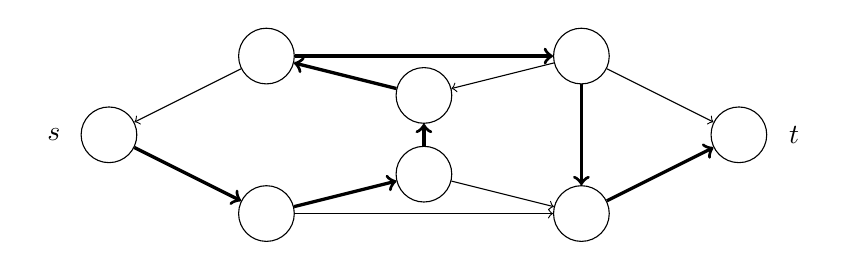
\begin{tikzpicture}
[inner sep=2.5mm]      
\path ( 0,1) node (0) [shape=circle,draw] {}
(2,2) node (1) [shape=circle,draw] {}
(2,0) node (2) [shape=circle,draw] {}
(4,1.5) node (3) [shape=circle,draw] {}
(4,0.5) node (4) [shape=circle,draw] {}
(6,2) node (5) [shape=circle,draw] {}
(6,0) node (6) [shape=circle,draw] {}
(8,1) node (7) [shape=circle,draw] {};
\path ( -0.7,1) node {$s$};
\path ( 8.7,1) node {$t$};
\draw [->] (1) -- (0);
\draw [->] (5) -- (3);
\draw [->] (5) -- (7);
\draw [->] (2) -- (6);
\draw [->] (4) -- (6);
\draw [->, very thick] (4) -- (3);
\draw [->, very thick] (0) -- (2);
\draw [->, very thick] (3) -- (1);
\draw [->, very thick] (1) -- (5);
\draw [->, very thick] (5) -- (6);
\draw [->, very thick] (2) -- (4);
\draw [->, very thick] (6) -- (7);
\end{tikzpicture}
\end{center}

\item $\text{HAMPATH}=\{\langle  G,s,t\rangle \mid G:$ directed,
a Hamiltonian path from $s$ to $t\}$
\item A brute-force way: checking all possible paths
\item [] But the number is exponential
\item Polynomial verification

\item [] for a path, in P time $\Rightarrow$ a Hamiltonian path or not

\item This is an example where verification is easier than determination

\end{itemize}\end{frame} \begin{frame}[allowframebreaks] \frametitle{Compositeness}
  \begin{itemize}
  \item We discuss another
    example where verification is easier than determination
  \item An integer is composite if
    \begin{equation*}
    x=pq, p > 1, q > 1
  \end{equation*}
\item Given $x$, difficult to find $p,q$

\item Given $x,p,q$ easily verify $x=pq $ or not
\end{itemize}\end{frame}

\begin{frame}[allowframebreaks] \frametitle{Not polynomial verifiable}
  \begin{itemize}
  \item Some problems are difficult so even a polynomial verifier cannot
    be easily obtained
\item $\overline{HAMPATH}$: given $\langle  G,s,t\rangle$ no Hamiltonian
path from $s$ to $t$

\item Verification may still be difficult
\item Given $s$ and $t$ it seems we 
still need to check all paths

\end{itemize}\end{frame} \begin{frame}[allowframebreaks] \frametitle{Verifier}
  \begin{itemize}
\item Definition: an algorithm V is a verifier of a language A if
  \begin{equation*}
    A=\{w\mid
V \mbox{ accepts } 
\langle  w,c\rangle  
\mbox{ for some strings } c\}
  \end{equation*}
\item Example: compositness. $V$ accepts $\langle  w,c\rangle  = \langle  x,p\rangle $, where $p$ is a divisor
\item Example: Hamiltonian path. $V$ accepts
  \begin{equation*}
  \langle  w,c\rangle  = \langle  \langle  G,s,t\rangle , \mbox{a path from $s$ to $t$}\rangle 
\end{equation*}
\item $c$ is called a  ``certificate''
\item Definition: a polynomial verifier if it takes polynomial time of $|w|$
\item A: polynomially verifiable if 
  $\exists$ a polynomial verifier
\item Note that we measure time on $|w|$ without considering $|c|$

\item For a polynomial verifier,  $|c|$ should be in polynomial of $|w|$

\item [] Otherwise, reading $|c|$ already non-polynomial
\end{itemize}\end{frame} \begin{frame}[allowframebreaks] \frametitle{NP}
  \begin{itemize}
\item NP is a class of languages 
\item Definition: a language $\in$ NP if it has a polynomial verifier
\item We will prove that this definition is equivalent to that the language
  is decided by nondeterministic polynomial TM 
\item This is where the name comes from

\item Some use this as the definition

\item Note that for nondeterministic TM time is by checking the longest branch

\item Definition:

  \begin{equation*}
    \begin{split}
      & \text{NTIME}(t(n)) \\
      =& \{L\mid L
\text{ decided by } O(t(n))
\text{ nondeterministic TM}\}
\end{split}
\end{equation*}
\item NP = $\cup_k \text{NTIME}(n^k)$

\end{itemize}\end{frame} \begin{frame}[allowframebreaks] \frametitle{NTM for HAMPATH}
  \begin{itemize}
\item A list $p_1\cdots p_m$ is nondeterministically determined

\item For each list:

  \begin{enumerate}
  \item  Check repetitions
  \item Check $s=p_1$; $t=p_m$
\item Check that for $1 \ldots m-1, (p_i, p_{i+1})$ is an edge of $G$
  \end{enumerate}
\item Cost on each list is polynomial:

  
\item [] repetitions: $O(m^2)$

\item [] $s=p_1, t = p_m: O(m)$

\item [] edge check: $O(m^2)$

\end{itemize}\end{frame}

\end{document}
